\documentclass{article}
\usepackage[utf8]{inputenc}
\usepackage{graphicx}

\title{SocialIqa_pt: A Translation of a Common-Sense Reasoning Dataset}
\author{Fabio Grassiotto}
\date{30 June 2024}

\begin{document}

\maketitle

\begin{abstract}
    The abstract is a short text to let people understand what is the document about.
    It should give the mains highlights of the documents.
    This document is a template to be use in the Final Project of the EA376E class.
    The recommendation is to use LaTeX by the application Overleaf.com, but it is also
    possible to use Google Docs or MS-Word.
\end{abstract}

\section{Introduction}

This is an example of paper citation: BERT~ is a transformer. T5 also uses transformers.

\cite{lee2023survey}
\cite{kocmi2023large}
\cite{choi2022curious}
\cite{krause2023commonsense}
\cite{sap2019socialiqa}
\cite{zellers2019recognition}

\section{Methodology} 

This is an example of inserting a figure. 

\begin{figure}[ht]
\centering
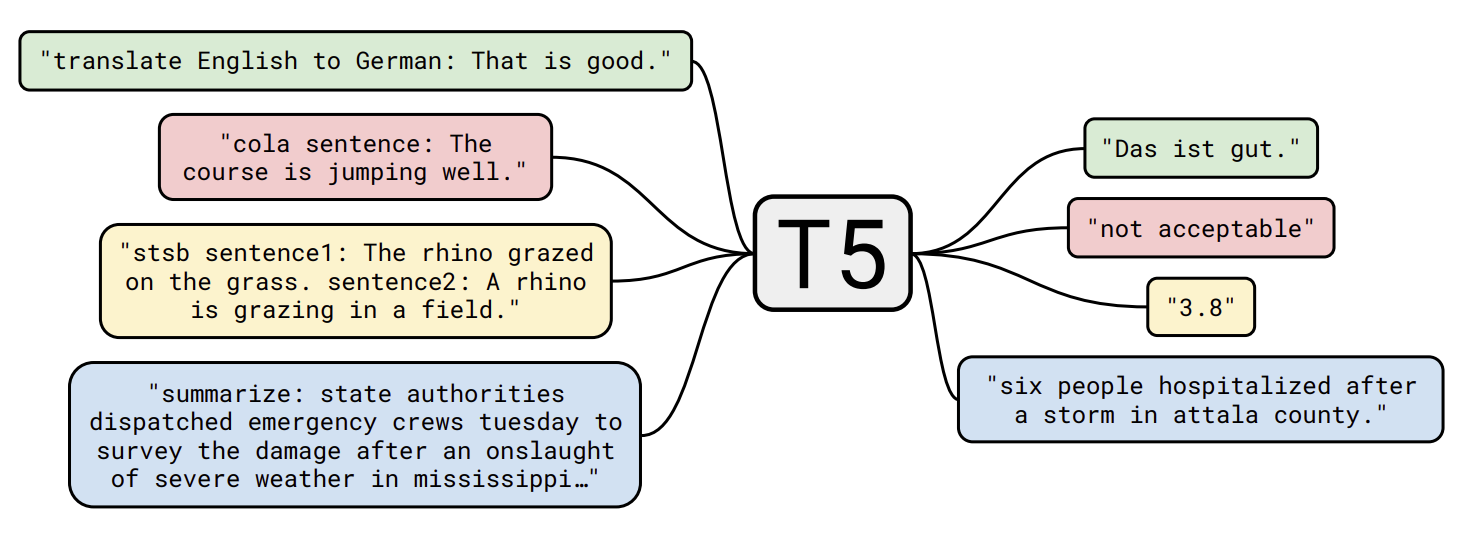
\includegraphics[width=.77\textwidth]{figures/t5.png}
\caption{\label{fig:t5}Figure example.}
\end{figure}

Figure~\ref{fig:t5} is an example of figure citation.

\section{Data set}

\section{Experiments}

\section{Conclusion}

\section{Future Work}

% Usando a bibliografia com arquivo no formato bibtex, (ver arquivo main.bib que faz parte desse projeto)
\bibliographystyle{plain}
\bibliography{main.bib}

\end{document}
